\section[Environment]{Environments and code checks}
\sectionframe{02}{Environments and code checks}
  {Where does the agent run our code, and what checks it automatically?}
  {\faCubes}

% ------------------------------------------------------------------ conda
\begin{frame}[fragile,source={conda (2026), Managing environments}]{The classic setup: a conda environment}
  \begin{columns}[T,onlytextwidth]
    \begin{column}{0.42\textwidth}
\begin{codefile}[style=sh,basicstyle=\ttfamily\fontsize{7.2}{8.8}\selectfont]{environment.yml}
name: sem-seg
channels:
  - conda-forge
dependencies:
  - python=3.12
  - numpy
  - pandas
  - pytorch      # with CUDA builds
  - pytest
\end{codefile}
      % uv as a link to its repository, styled as the one over the screenshot on slide 28
      {\footnotesize Python-only projects:
       \href{https://github.com/astral-sh/uv}{\faGithub\enspace\underline{\fn{uv}}} is faster\par}
    \end{column}
    \begin{column}{0.55\textwidth}
\begin{terminal}[basicstyle=\ttfamily\fontsize{7.2}{8.8}\selectfont]{terminal}
$ conda env create -f environment.yml
$ conda activate sem-seg
$ conda run -n sem-seg pytest -q    # no activation
\end{terminal}
      \vskip1.4mm
      % an agent runs each command in a new shell, so an activation does not carry over
      \begin{tikzpicture}[x=1mm,y=1mm,
          sh/.style={anchor=west,inner sep=0pt,font=\ttfamily\fontsize{7}{8}\selectfont,text=termfg,
            execute at begin node={\setbox0\hbox{x}\spaceskip=\wd0\relax}},
          env/.style={anchor=west,rounded corners=0.8mm,inner xsep=1.1mm,inner ysep=0.7mm,
            font=\ttfamily\fontsize{7}{8}\selectfont\bfseries,text=white}]
        \node[anchor=north west,inner sep=0pt,font=\footnotesize\bfseries,text=udsdark] at (0,0)
          {an agent session: a new shell for every command};
        \foreach \i/\c/\e/\col in {1/{conda activate sem-seg}/{sem-seg}/udsblue,
            2/{pytest -q}/{not sem-seg}/udsred,3/{conda run -n sem-seg pytest -q}/{sem-seg}/udsblue} {
          \pgfmathsetmacro\y{-1.8-\i*6.2}
          \fill[termbg,rounded corners=1mm] (0,\y+2.4) rectangle (57,\y-2.4);
          \foreach \d [count=\j] in {termdot1,termdot2,termdot3} \fill[\d] (\j*1.7,\y) circle (0.45);
          \node[sh] at (6.8,\y) {\textcolor{termgreen}{\$} \c};
          \node[env,fill=\col] at (59,\y) {\e};
        }
      \end{tikzpicture}\par\vskip1.4mm
      {\footnotesize or: activate first, then start the agent\par}
    \end{column}
  \end{columns}
  \note{\textbf{6:00--7:00}\par
    Most of us use conda.\par
    An environment.yml lists channel and packages; conda builds the environment, activate enters it.\par
    Three things matter once an agent works in it.\par
    Each command an agent runs starts a fresh shell, so an activation does not carry over;
      Claude Code's documentation says to activate the environment before launching it, and
      conda run executes a command in an environment without activating it.\par
    An environment.yml without versions drifts: rebuilt next year, it resolves to different
      packages; conda 26.5 and later export a lockfile with exact versions, conda-lock does the
      same for older versions.\par
    And the channel: PyTorch's conda packages now come from conda-forge, Miniforge's only channel.\par
    Anaconda's own channel has terms of service, free for academic use under conditions, that
      count AI agents and automated jobs as users; check with the university's IT before relying
      on it.\par
    For Python-only projects uv is faster; A3 and A4 in the appendix show it.}
\end{frame}

% ------------------------------------------------------------ three tools
% One card per tool: its job, the kind of tool, a small example drawn as an editor shows it (a
% wavy red line under a finding) and where it runs; the strip says how the three combine.
\begin{frame}[source={Astral (2026), Ruff documentation · mypy documentation · Microsoft (2026), Pylance README}]{Ruff, mypy and Pylance}
  \begin{tikzpicture}[x=1mm,y=1mm,
      toolname/.style={anchor=west,inner sep=0pt,font=\small\bfseries,text=white},
      job/.style={anchor=base west,inner sep=0pt,font=\footnotesize\bfseries,text=udsdark},
      kind/.style={anchor=base west,inner sep=0pt,font=\scriptsize,text=udsgrey},
      code/.style={anchor=base west,inner sep=0pt,font=\ttfamily\fontsize{7}{8}\selectfont,
        text=udsdark,execute at begin node={\setbox0\hbox{x}\spaceskip=\wd0\relax}},
      tag/.style={anchor=base west,inner sep=0pt,font=\scriptsize},
      squiggle/.style={udsred,line width=0.45pt,decorate,
        decoration={snake,amplitude=0.22mm,segment length=1.1mm}},
      chip/.style={draw=udsgreylight,fill=white,rounded corners=0.6mm,inner xsep=1mm,
        inner ysep=0.6mm,anchor=west,font=\scriptsize,text=udsdark}]
    \useasboundingbox (0,0) rectangle (144,-55);
    % three cards, 46 mm wide and 3 mm apart, each with a code window and where the tool runs
    \foreach \x/\icon/\n in {0/\faSpellCheck/Ruff,49/\faPuzzlePiece/mypy,98/\faKeyboard/Pylance} {
      \fill[udsblue] (\x,0) rectangle (\x+46,-6.2);
      \fill[bluetint] (\x,-6.2) rectangle (\x+46,-44.6);
      \node[toolname] at (\x+2.2,-3.1) {\icon\enspace\n};
      \filldraw[fill=white,draw=udsgreylight,line width=0.4pt,rounded corners=0.8mm]
        (\x+2.2,-17.6) rectangle (\x+43.8,-35.4);
      \node[kind,anchor=west] at (\x+2.2,-40.4) {runs in};
      \node[chip] (vs\x) at (\x+12,-40.4) {\faCode\enspace VS Code};
    }
    \foreach \x in {0,49} \node[chip] at ([xshift=1.5mm]vs\x.east) {\faTerminal\enspace terminal};
    % Ruff: an unused import, flagged; a line laid out again
    \node[job] at (2.2,-11.2) {how the code is written};
    \node[kind] at (2.2,-15.1) {linter and formatter};
    \node[code] at (4,-22.4) {import os};
    \draw[squiggle] (4,-23.6) -- (15.7,-23.6);
    \node[tag,text=udsred] at (18,-22.4) {unused import};
    \node[code] at (4,-30.4) {x=[1,2 ,3]};
    \draw[flow,draw=udsgreymid] (18.2,-29.6) -- (21.8,-29.6);
    \node[code,text=testgreen] at (23,-30.4) {x = [1, 2, 3]};
    % mypy: the same type hint, met by a number and broken by text
    \node[job] at (51.2,-11.2) {whether the types match};
    \node[kind] at (51.2,-15.1) {type checker: reads the type hints};
    \node[code] at (53,-22.4) {n\_folds: int = 3};
    \node[tag,text=testgreen] at (76,-22.4) {\faCheck};
    \node[code] at (53,-30.4) {n\_folds: int = "3"};
    \draw[squiggle] (72.5,-31.6) -- (76.4,-31.6);
    \node[tag,text=udsred] at (78.4,-30.4) {not an int};
    % Pylance: what the function expects, shown while the call is typed
    \node[job] at (100.2,-11.2) {help while you type};
    \node[kind] at (100.2,-15.1) {VS Code's language server};
    \node[code] at (102,-22.4) {specimen\_folds(};
    \draw[udsdark,line width=0.5pt] (121.9,-23.1) -- (121.9,-19.9);
    \node[code,anchor=north west,fill=white,draw=udsgreylight,line width=0.4pt,inner xsep=1mm,
      inner ysep=0.8mm] at (103,-24.2) {(\textcolor{udsblue}{\textbf{manifest}}, n\_folds: int)};
    \node[tag,text=udsgrey] at (102,-33.4) {and type checks, once switched on};
    % how the three combine
    \fill[bluetint] (0,-48.4) rectangle (144,-54.6);
    \fill[udsblue] (0,-48.4) rectangle (1.2,-54.6);
    \node[anchor=west,inner sep=0pt,font=\footnotesize,text=udsdark] at (3.6,-51.5)
      {\textbf{together:}\enspace Pylance while you write; Ruff and mypy as the checks you and the
       agent run};
  \end{tikzpicture}
  \note{\textbf{7:00--8:00}\par
    Three tools that read the code without running it, each with its own job.\par
    Ruff checks how the code is written: it flags likely mistakes, such as an import that is
      never used, and lays the code out the same way every time; a spell checker and a
      typesetter for code.\par
    mypy checks whether the types match: with the hint n\_folds: int, the number 3 passes and
      the text ``3'' does not, much as the units in an equation must match.\par
    Pylance is VS Code's language server: it completes names, shows what a function expects as
      you type and jumps to definitions; once its type checking is switched on, it checks types
      too, as you type.\par
    Ruff and mypy run in VS Code and in the terminal, so an agent can run them too; Pylance runs
      only in Microsoft's VS Code.\par
    So we use all three: Pylance while writing, Ruff and mypy as the checks before a change
      counts as done.}
\end{frame}

% ---------------------------------------------------------- in VS Code
\begin{frame}{What it looks like in VS Code}
  \begin{columns}[T,onlytextwidth]
    \begin{column}{0.7\textwidth}
      \begin{tikzpicture}
        \node[anchor=south west,inner sep=0pt,draw=udsgreylight,line width=0.4pt] (img) at (0,0)
          {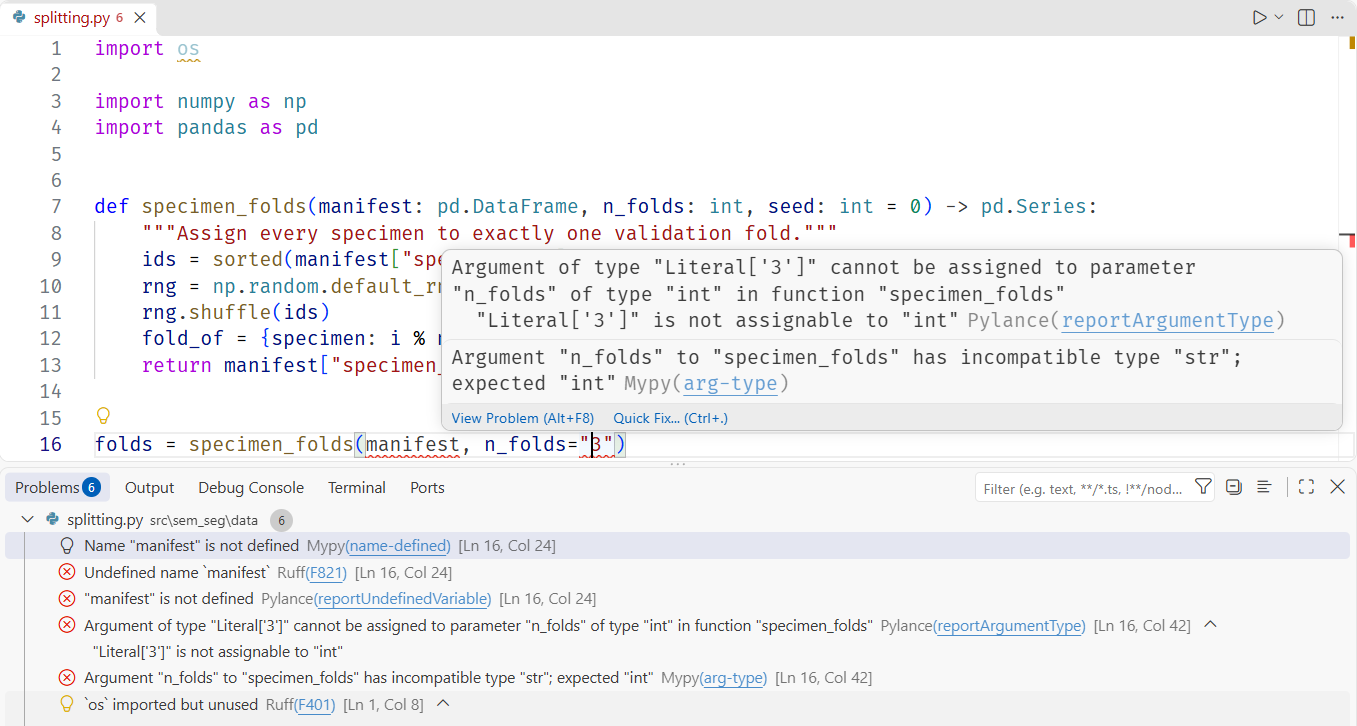
\includegraphics[width=\linewidth]{assets/screens/vscode-lint.png}};
        \begin{scope}[x={(img.south east)},y={(img.north west)}]
          \node[number mark] at (0.179,0.963) {1};
          \node[number mark] at (0.849,0.698) {2};
          \node[number mark] at (0.111,0.328) {3};
        \end{scope}
      \end{tikzpicture}
    \end{column}
    \begin{column}{0.27\textwidth}
      % each item numbered by its marker on the screenshot
      \footnotesize
      \begin{itemize}\setlength\itemsep{2mm}
        \item[\numbermark{1}] Ruff: unused import (\fn{F401}), undefined name (\fn{F821})
        \item[\numbermark{2}] Pylance and mypy: a string passed as \fn{n\_folds}
        \item[\numbermark{3}] Problems panel: every finding, with its tool and rule
      \end{itemize}
    \end{column}
  \end{columns}
  \note{\textbf{8:00--8:40}\par
    A real screenshot: VS Code 1.142 with the Ruff, Pylance and Mypy extensions on a
      deliberately broken version of our split function.\par
    Squiggles mark the unused import, the undefined name and the wrong argument type; hovering
      shows the message and which tool raised it.\par
    The Problems panel lists all six findings, each with its tool and rule, so you can look up
      or switch off a rule.\par
    The agent sees the same findings when it runs the tools from the terminal.}
\end{frame}

% ------------------------------------------------------------ set up once
\begin{frame}[fragile,source={Astral (2026), Ruff: editor setup · Microsoft (2026), Mypy Type Checker; Pylance README}]{Set them up once}
  % left: the tools on the command line; right: the same tools in VS Code. The right column is
  % wide enough for the longest line of settings.json (55 characters at 7 pt) on one line; the
  % left one then holds 42 characters of code and a table whose widest label is "Format".
  \begin{columns}[T,onlytextwidth]
    \begin{column}{0.425\textwidth}
\begin{codefile}[style=sh,basicstyle=\ttfamily\fontsize{7}{8.4}\selectfont]{pyproject.toml}
[tool.ruff]  # rules: Ruff's defaults
line-length = 100

[tool.mypy]
python_version = "3.12"
\end{codefile}
      \scriptsize\renewcommand\arraystretch{1.4}\setlength\tabcolsep{3pt}
      \begin{tabularx}{\linewidth}{@{}>{\bfseries}l>{\ttfamily}X@{}}
        \toprule
        Install        & conda install -c conda-forge ruff mypy\\
        \midrule
        Lint           & ruff check --fix\\
        Format         & ruff format\\
        Types          & mypy src\\
        \bottomrule
      \end{tabularx}
    \end{column}
    \begin{column}{0.545\textwidth}
\begin{codefile}[basicstyle=\ttfamily\fontsize{7}{8.4}\selectfont]{.vscode/settings.json}
{
  "[python]": {
    "editor.defaultFormatter": "charliermarsh.ruff",
    "editor.formatOnSave": true,
    "editor.codeActionsOnSave": {
      "source.fixAll": "explicit",
      "source.organizeImports": "explicit"}},
  "python.analysis.typeCheckingMode": "standard",
  "mypy-type-checker.importStrategy": "fromEnvironment"
}
\end{codefile}
      \footnotesize
      \begin{itemize}\setlength\itemsep{1mm}
        \item VS Code extensions: Python (brings Pylance), Ruff, Mypy Type Checker
        \item pick the environment: \emph{Python: Select Interpreter}
        \item the same commands go into \fn{AGENTS.md}
      \end{itemize}
    \end{column}
  \end{columns}
  \note{\textbf{8:40--9:40}\par
    Set up once per repository, then it runs by itself.\par
    The tool settings live in pyproject.toml, which works for conda projects too.\par
    One conda command installs both; by hand, three commands lint, format and type-check.\par
    In VS Code, install the Python extension, which brings Pylance, plus the Ruff and Mypy Type
      Checker extensions, and select the project's environment.\par
    The workspace settings make Ruff format and fix on every save, switch Pylance's type
      checking on, and make the Mypy extension use the mypy installed in the environment rather
      than the older copy it bundles.\par
    The same commands go into AGENTS.md, so the agent runs them too.}
\end{frame}
